\section{Affine curvature simulations}\label{sec:promasens:ac_simulations}
To demonstrate the efficacy of the proposed method for higher-order kinematic models than PCC, we also conduct simulations of an affine curvature soft robot.
The affine curvature kinematic parametrization~\cite{della2020soft} has been shown capable of representing the shape of soft tentacles~\cite{stella2022experimental, stella2022piecewise_preprint} and provides a continuous function $\kappa = \kappa_0 + \kappa_1 \: v$ to describe the curvature of the soft robot, where $\kappa_0$, $\kappa_1$ are two configuration variables and $v \in [0, 1]$ is the backbone coordinate. We allow for movement in 3D space by also specifying an azimuth bending angle $\phi$ and the elongation $\delta L$.
Please refer to Appendix~\ref{sub:promasens:kinematic_model_ac} for more implementation details about the affine curvature model.


\subsection{Simulation setup}\label{sub:promasens:ac_simulations:simulation_setup}
We use the same simulation setup as described in Section~\ref{sub:promasens:pcc_simulations:simulation_setup}. 
Therefore, we report in the following only the implemented modifications to simulate an affine curvature soft robot in Magpylib~\cite{magpylib2020}.
Namely, we consider one affine curvature segment of length $L_{0,i} = \SI{200}{mm}$ with in total $n_\mathrm{s} = 9$ magnetic sensors. 
The sensors are placed on three separate cylindrical planes at distances $d_{\mathrm{s}_\mathrm{a}}$ of \SI{0}{mm}, \SI{100}{mm}, and \SI{200}{mm} from the base of the robot. In each plane, the three sensors are spaced at an angle of \SI{120}{\degree} and at a radial distance $d_{\mathrm{s}_\mathrm{r}} = \SI{13}{mm}$ from the backbone, as it can be seen in Fig.~\ref{fig:promasens:ac_simulations:inference_sequences}.
Two ring magnets are positioned at a distance of \SI{50}{mm} and \SI{150}{mm} from the robot's base respectively.

\begin{figure}[hbt]
  \centering
  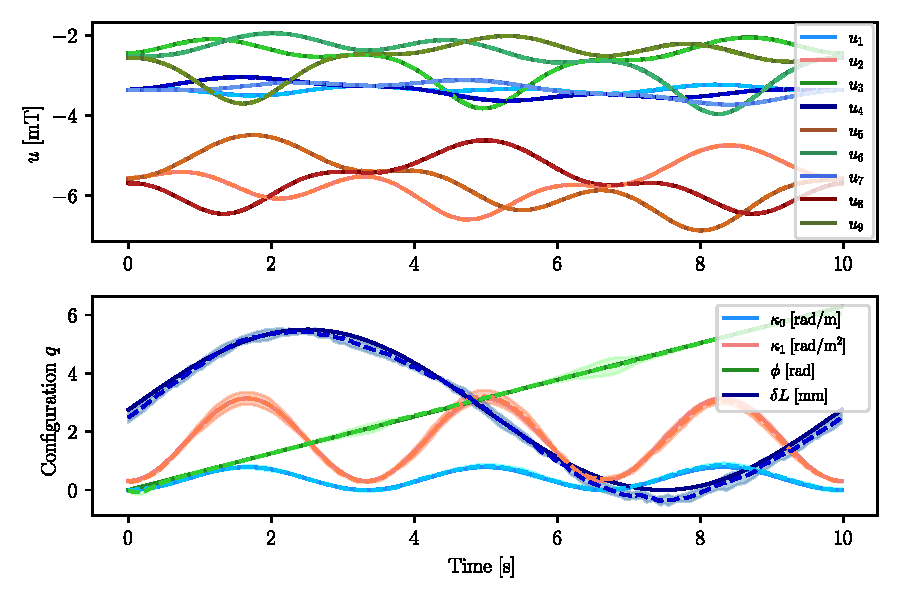
\includegraphics[width=1.0\columnwidth]{promasens/figures/simulation_results/ac/affine_curvature_inference_v2_cropped.pdf}
  \caption{Sensor measurement predictions (top) and configuration estimates (bottom) for an affine curvature segment with nine magnetic sensors. We plot the ground-truth values $u$ and $q$ in solid, the estimate $\hat{u}$ and $\hat{q}$ as a mean over three random seeds with dashed lines and the standard deviation as an error band. The random seed determines at the start of the training the initialization of the neural network weights.}
  \label{fig:promasens:ac_simulations:inference_plot}
\end{figure}

\begin{figure*}[hbt]
  \centering
  \subfloat[$t=\SI{0}{s}$]{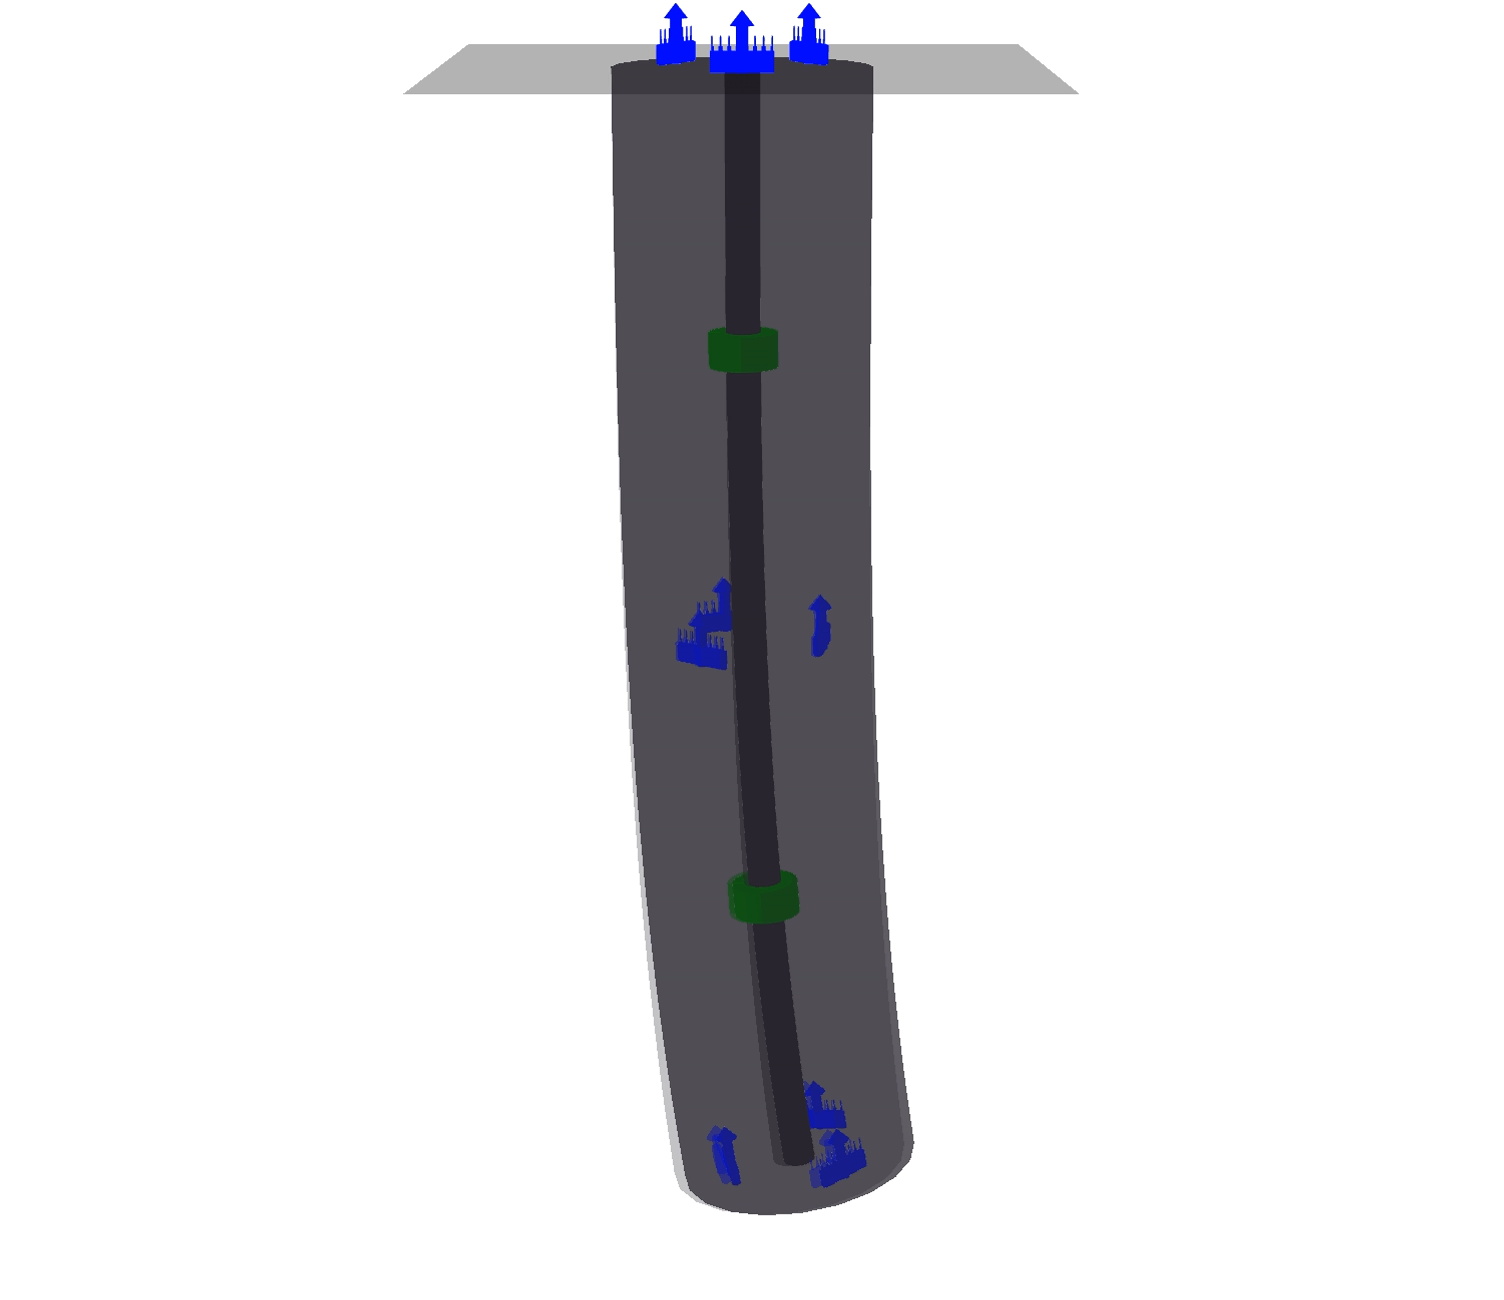
\includegraphics[width=0.162\textwidth]{promasens/figures/simulation_sequences/ac_flower_trajectory/affine_curvature_flower_t=0s_cropped.png}}
  \hfill
  \subfloat[$t=\SI{2}{s}$]{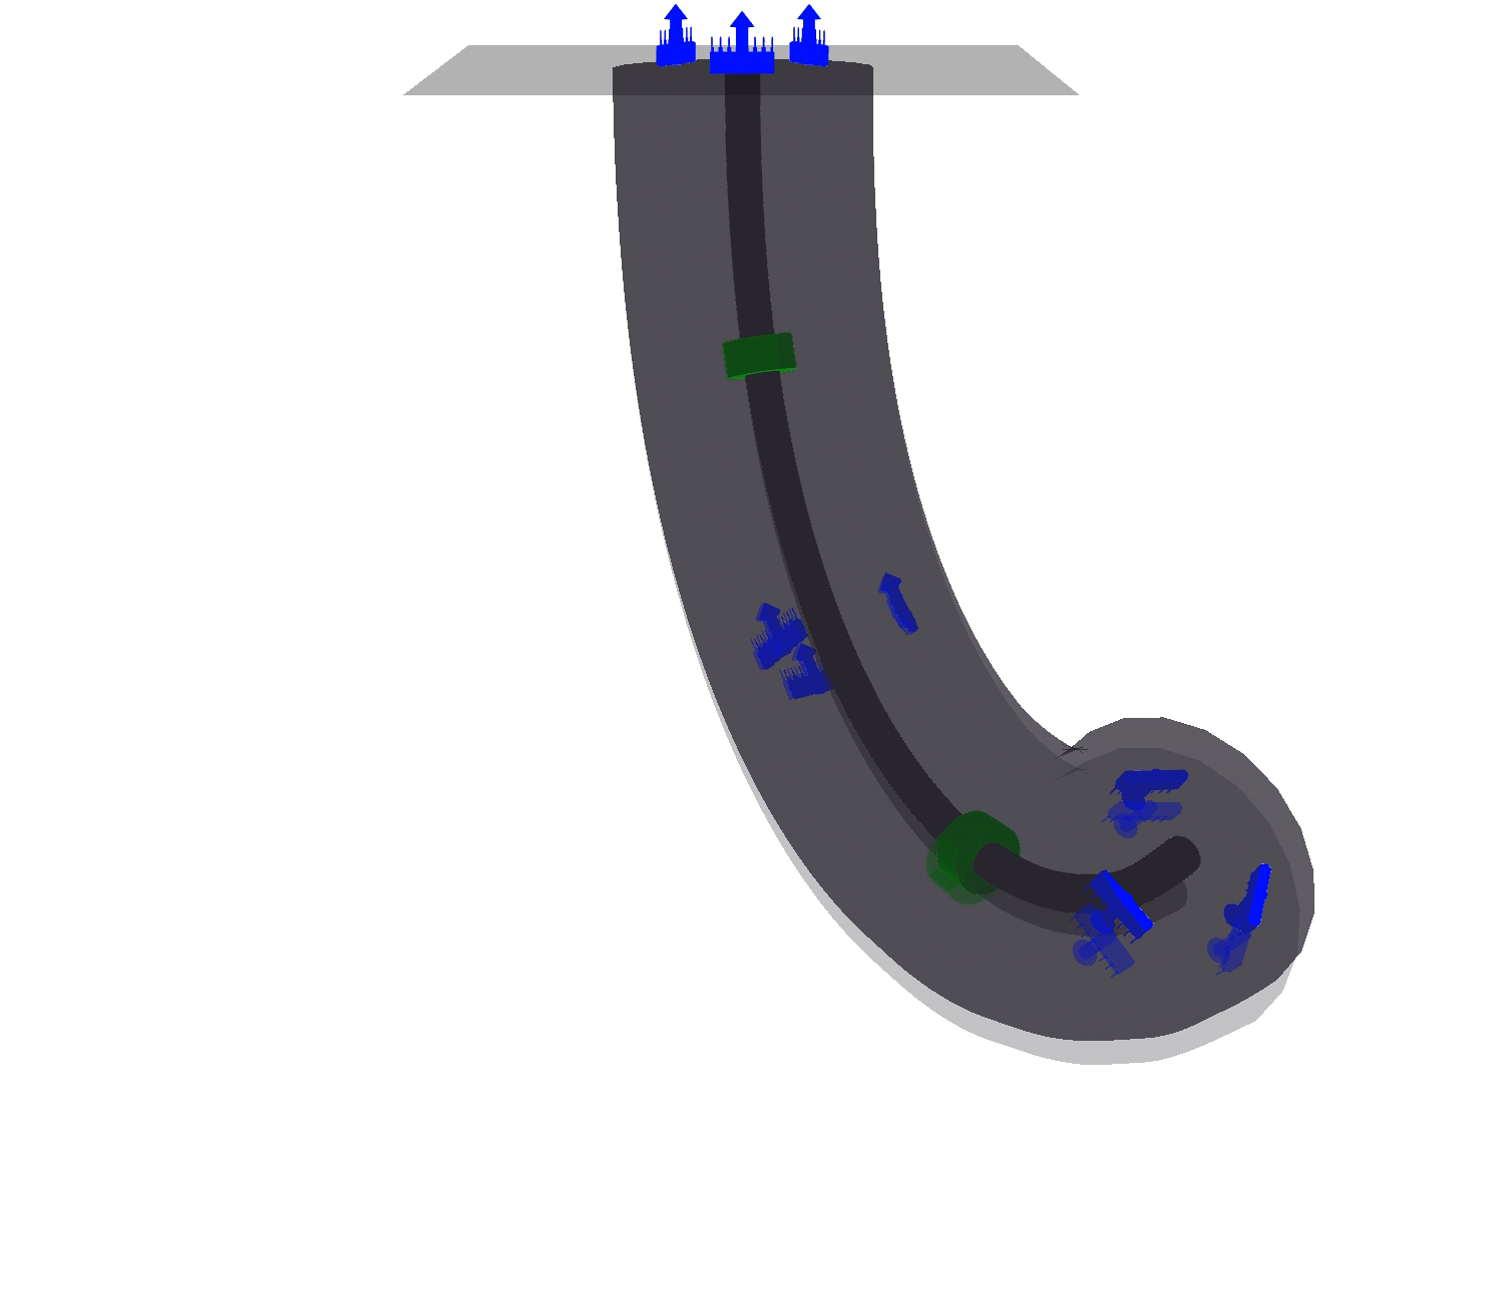
\includegraphics[width=0.162\textwidth]{promasens/figures/simulation_sequences/ac_flower_trajectory/affine_curvature_flower_t=2s_cropped.png}}
  \hfill
  \subfloat[$t=\SI{4}{s}$]{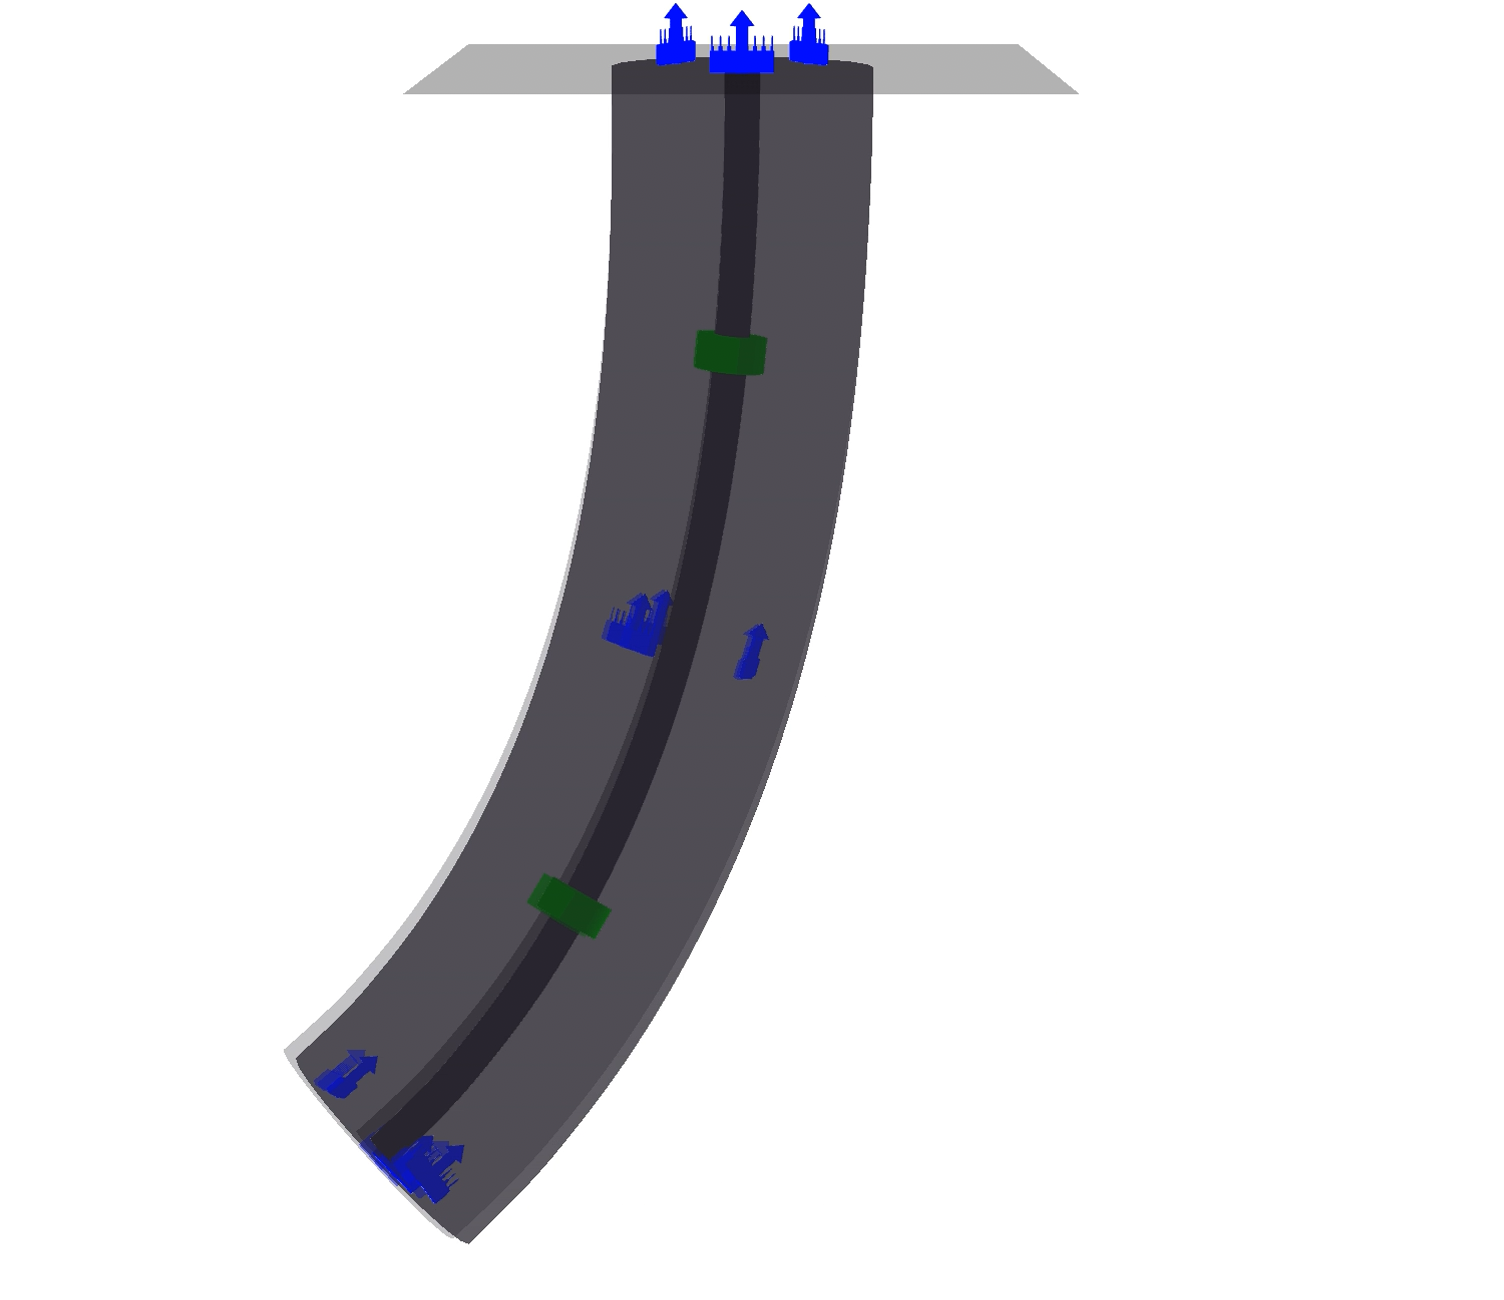
\includegraphics[width=0.162\textwidth]{promasens/figures/simulation_sequences/ac_flower_trajectory/affine_curvature_flower_t=4s_cropped.png}}
  \hfill
  \subfloat[$t=\SI{6}{s}$]{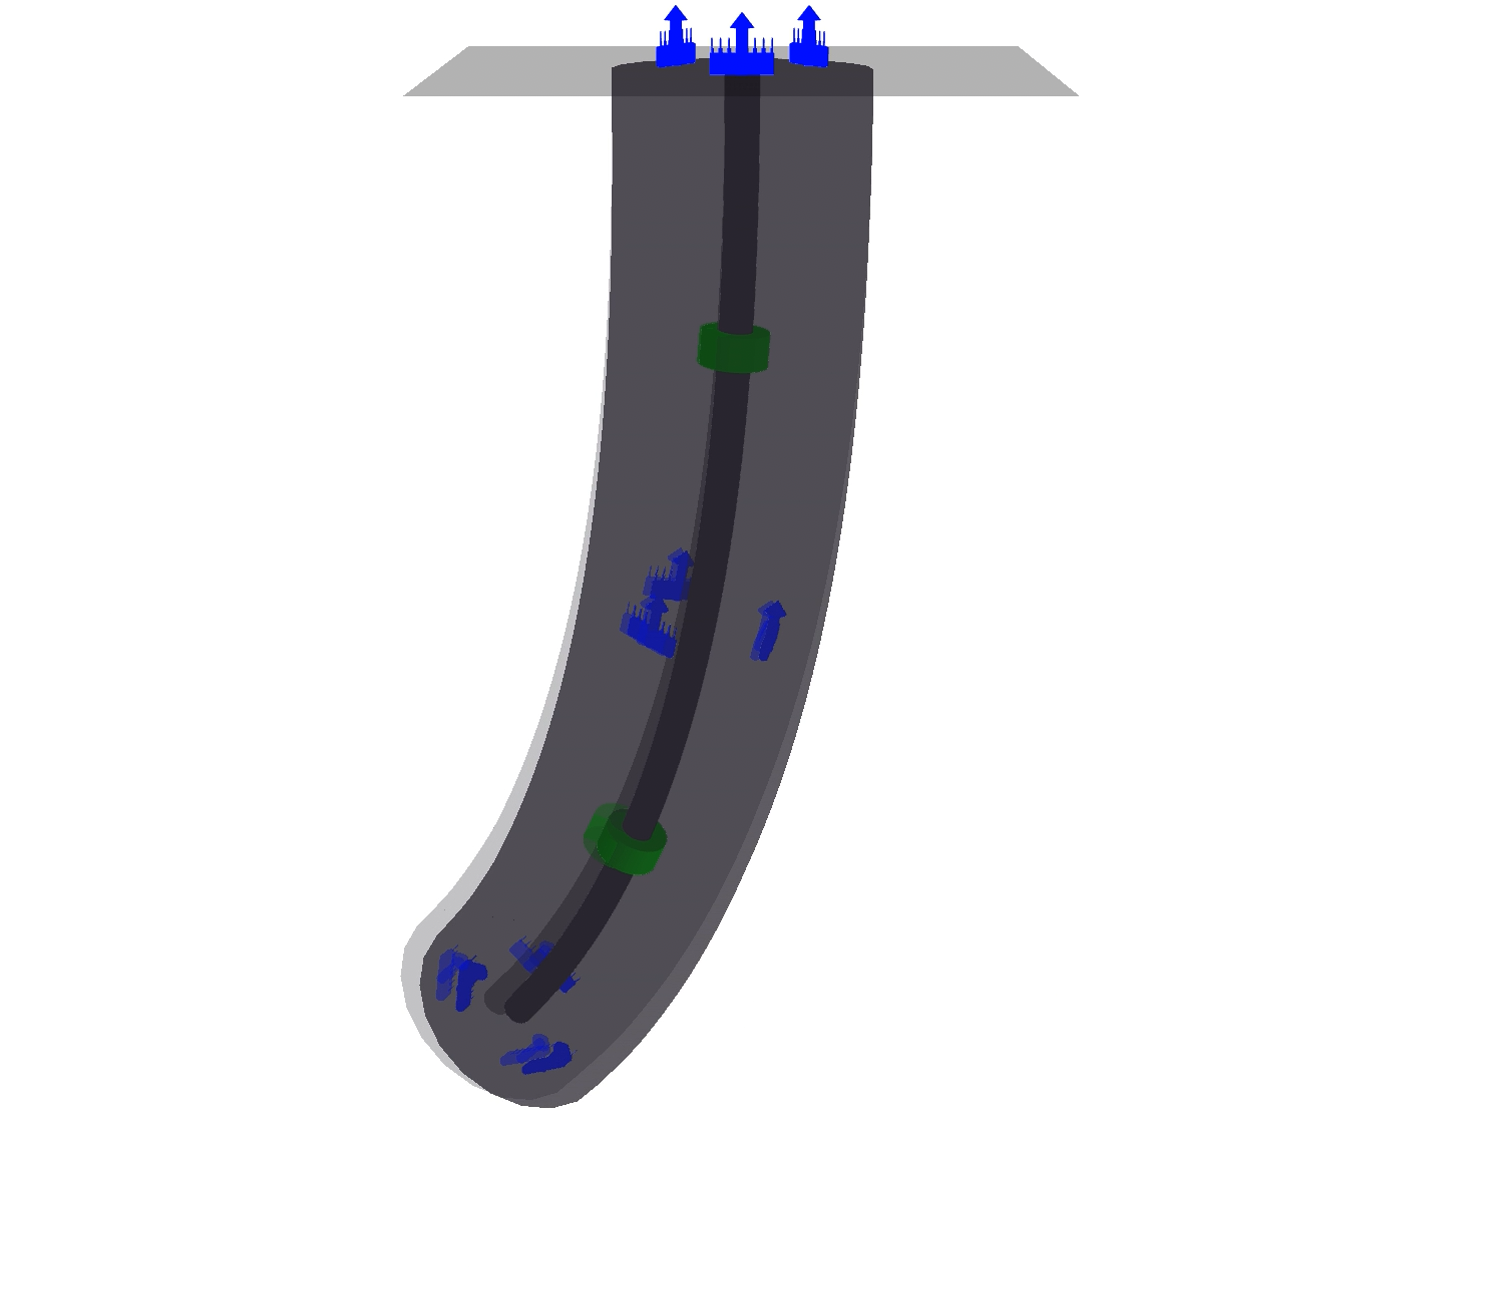
\includegraphics[width=0.162\textwidth]{promasens/figures/simulation_sequences/ac_flower_trajectory/affine_curvature_flower_t=6s_cropped.png}}
  \hfill
  \subfloat[$t=\SI{8}{s}$]{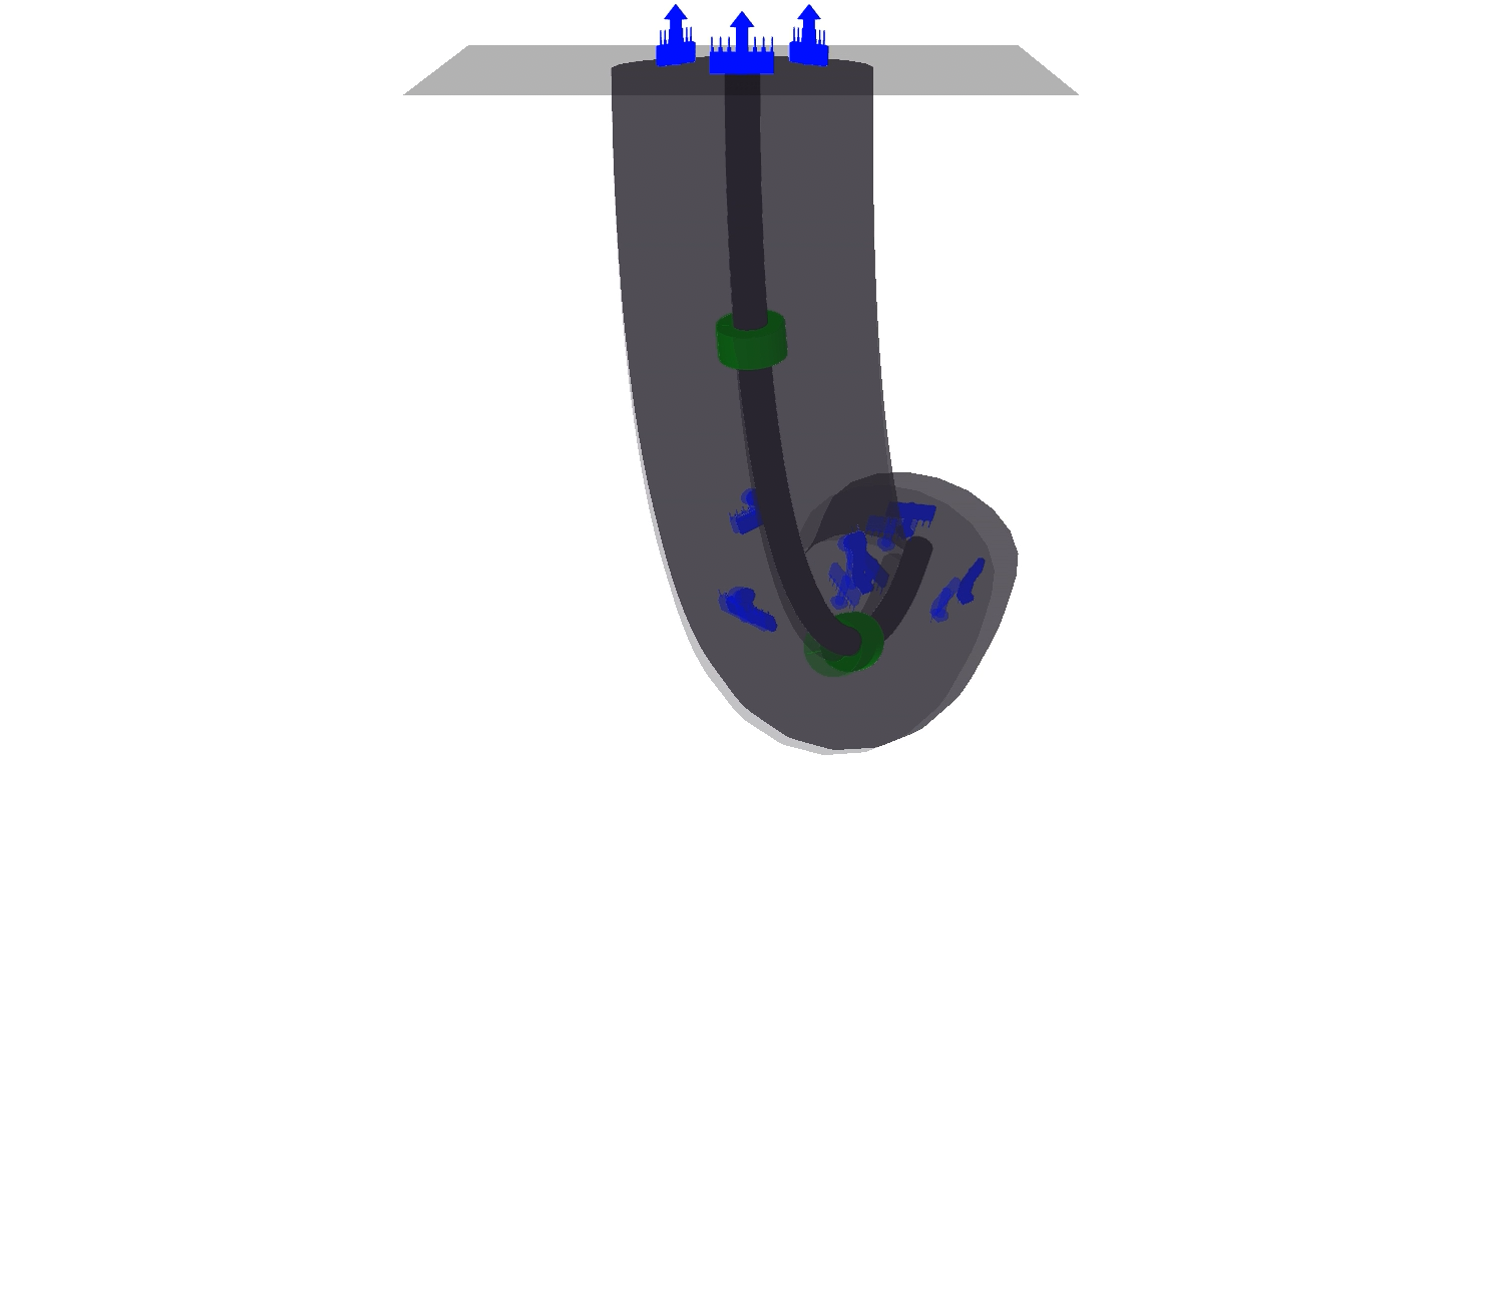
\includegraphics[width=0.162\textwidth]{promasens/figures/simulation_sequences/ac_flower_trajectory/affine_curvature_flower_t=8s_cropped.png}}
  \hfill
  \subfloat[$t=\SI{10}{s}$]{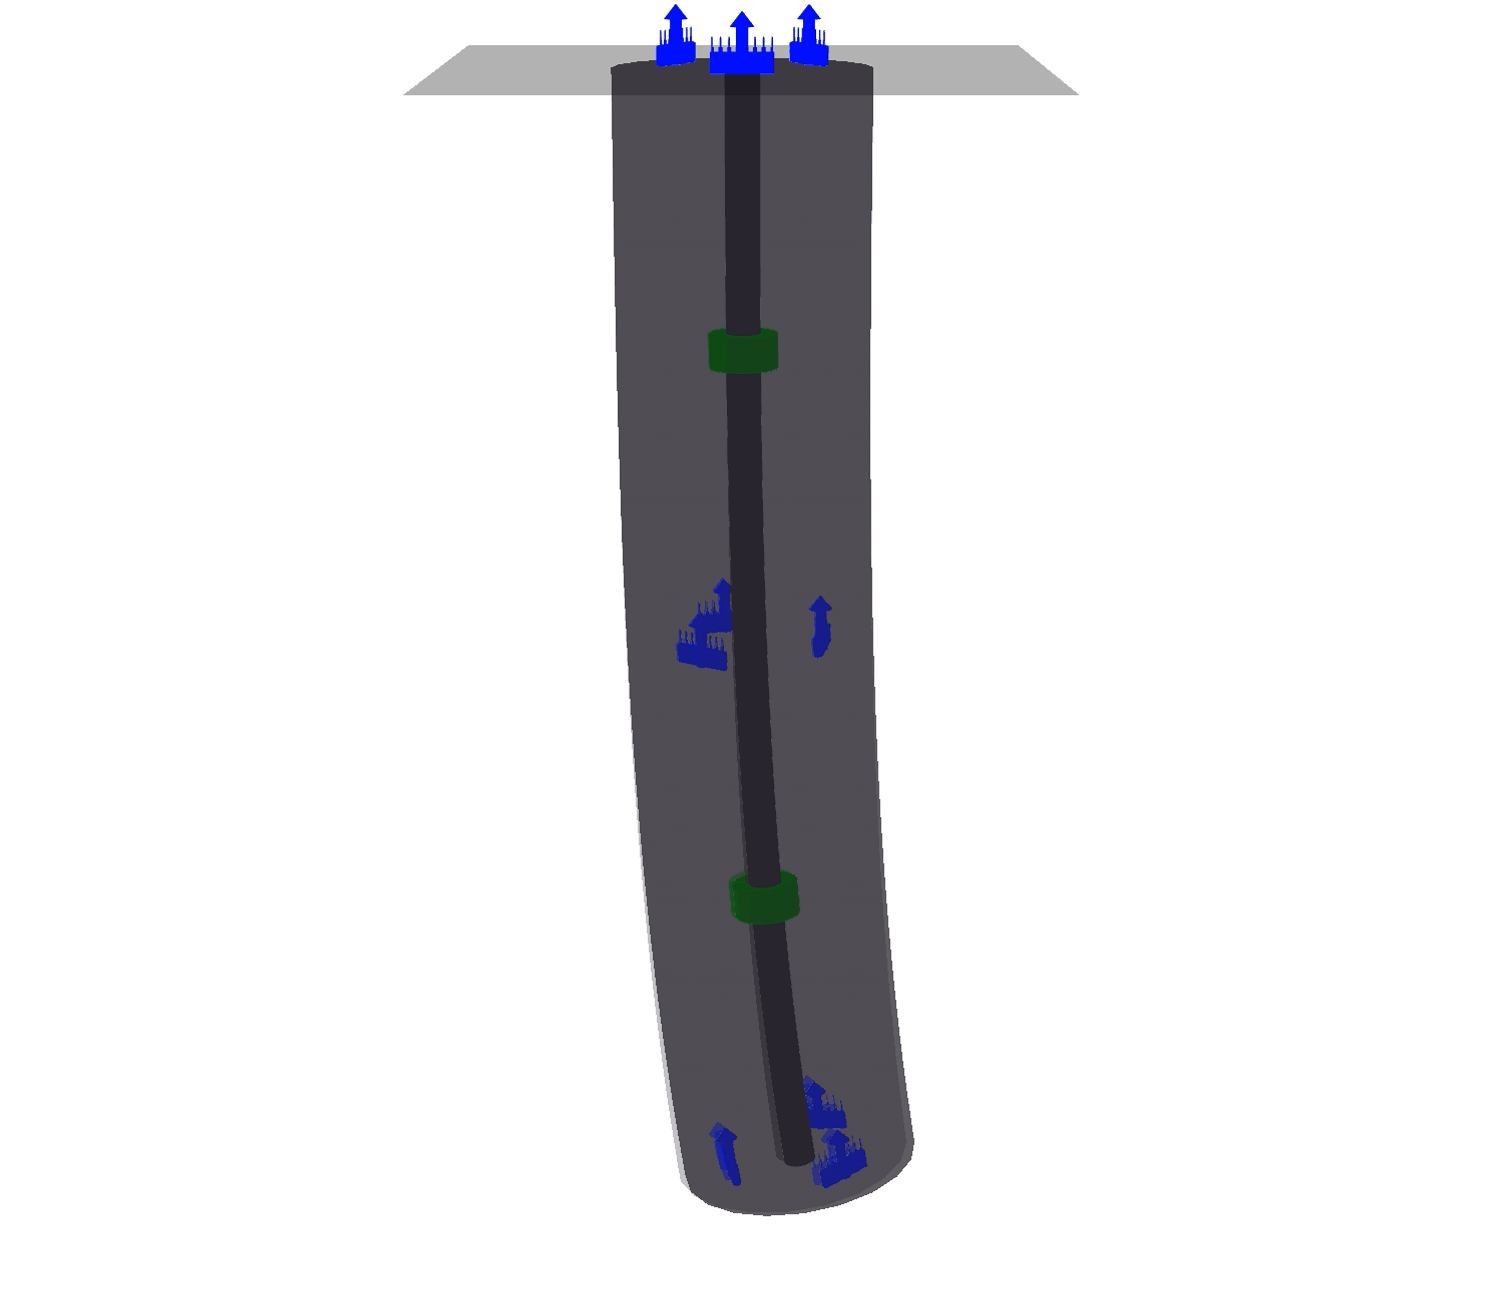
\includegraphics[width=0.162\textwidth]{promasens/figures/simulation_sequences/ac_flower_trajectory/affine_curvature_flower_t=10s_cropped.png}}
  % 1504 x 1400px
  \caption{Sequence of stills for a simulated affine curvature robot. We visualize the ground-truth shape of the soft robot with full opacity and the estimated configuration with slight transparency. The two magnets are rendered in green and the nine sensors in blue.}
  \label{fig:promasens:ac_simulations:inference_sequences}
\end{figure*}

\subsection{Prediction network and optimization}\label{sub:promasens:ac_simulations:network_optimization}
We simulate \SI{120000}{} random configurations of the affine curvature robot to generate the training set. For this purpose, we sample the configuration variables from uniform distributions: the affine curvature parameters $\kappa_0 \in \mathcal{U}(0, \SI{0.942}{rad \per m})$, $\kappa_1 \in \mathcal{U}(0, \SI{3.770}{rad \per m^2})$, the azimuth angle $\phi \in \mathcal{U}(0, 2 \pi \: \si{rad})$, and the elongation $\delta L \in \mathcal{U}(0, \SI{6.6}{mm})$.
Before training, we randomly split off \SI{30}{\percent} of the training set for validation purposes.
We train a specialized neural network $f_{\pi_j(\xi_j)}$ for each sensor and use the same neural network architecture as in Section~\ref{sub:promasens:pcc_simulations:neural_network} with the exception of the addition of a final layer $y(x) = \mathrm{sign}(x) \: e^{|x|}$. 
The training runs for in total $250$ epochs and uses the SWA~\cite{izmailov2018averaging} strategy with a learning rate of $0.01$. 
All other training hyperparameters are the same as in Section~\ref{sub:promasens:pcc_simulations:neural_network}.

The four configuration variables are optimized to minimize the loss between the predictions and simulated measurements of the nine sensors as defined in \ref{eq:promasens:proprioception_loss}.
For this optimization procedure, we employ gradient descent running at \SI{40}{Hz} with step sizes of $\gamma_{\kappa_0} = 1$, $\gamma_{\kappa_1} = 5$, $\gamma_{\phi} = 1$, and $\gamma_{\delta L} = 2 \cdot 10^{-4}$. The momentum is set to $\mu = 0.3$ and $20$ iterations are performed at each time step.

\subsection{Evaluation}\label{sub:promasens:ac_simulations:evaluation}
We evaluate the trained model on a flower trajectory of duration \SI{10}{s} and sample rate \SI{40}{Hz}. The evaluation trajectory has the following characteristics: $\kappa_0$ is actuated by a sinusoidal wave of frequency \SI{0.3}{Hz} in the range $[0, \frac{\pi}{4} \: \si{rad \per m}]$. Similarly, $\kappa_1$ is also varied through a sinusoidal function of the same frequency and has a dynamic range of $[0.1 \pi, \pi] \: \si{rad \per m^2}$.
The azimuth angle $\phi$ is linearly scaled from \SI{0}{rad} to $2 \pi \: \si{rad}$ over the duration of the trajectory.
Finally, $\delta L$ follows a sinusoidal sequence of frequency \SI{0.1}{Hz} in the range of $[0, 5.5] \: \si{mm}$.
We use the same evaluation metrics as first introduced in Section~\ref{sub:promasens:pcc_simulations:evaluation}.
We report the error as mean ± stdev and compute the statistics over three
different random seeds. The random seed determines at the start of the training the initialization of the neural network weights.

\subsection{Results}\label{sub:promasens:ac_simulations:results}
The trained neural networks achieve an RMSE error for predicting the magnetic sensor measurements of $0.025 \pm 0.002 \: \si{mT}$ on the test set.
When we run inference (see Fig.~\ref{fig:promasens:ac_simulations:inference_plot}) on the flower trajectory, the configuration variables can be estimated with an absolute RMSE of $e_{\kappa_0} = 0.042 \pm 0.005 \: \si{rad \per m}$, $e_{\kappa_1} = 0.11 \pm 0.04 \: \si{rad \per m^2}$, $e_{\phi} = 0.08 \pm 0.02 \: \si{rad}$, and $e_{\delta L} = 0.001 \pm 0.001 \: \si{mm}$. 
We state the relative RMSE errors for the configuration estimates as $e_{\kappa_0} = 5.4 \pm 0.7 \: \si{\percent}$, $e_{\kappa_1} = 4.0 \pm 1.4 \: \si{\percent}$, $e_{\phi} = 1.3 \pm 0.4 \: \si{\percent}$, and $e_{\delta L} = 3.8 \pm 1.6 \: \si{\percent}$.
In Fig.~\ref{fig:promasens:ac_simulations:inference_sequences}, we render at six different points along the trajectory the robot's shape according to the ground truth and estimated configurations respectively.
The sequence qualitatively shows that our proposed method is able to estimate the affine curvature robot's shape very accurately.
